\documentclass[bsc,m,palatino,oneside,12pt]{softlang}

% Use one of the following terms and replace msc as argument in documentclass:
% Master of Science thesis: msc
% Bachelor of Science thesis: bsc
% Projektpraktikum: pp
% Diplomarbeit: diplom
% Proseminar: prosem
% Seminararbeit: sem
% Skript: scr
% Studienarbeit: sa

% Use m(Männlich) or w(Weiblich) as argument in documentclass
% 12pt is the size of the text
% oneside is for normal text layout, the text is centered
% twoside prints the text assymmetric
% palatino is tzhe font of the letters


% BibLatex for Bibliography
% For Citation- and Bibliographystyles refer to the biblatex documentation
% Standard is numeric both
\usepackage{biblatex}
\addbibresource{bibliography.bib}

% This are optional packages, to use them remove the %:
\usepackage{booktabs} %for optimicing tabulars
%\usepackage{bibgerm} % for german BibTex styles
\usepackage{wrapfig}% for wrapping text arount tables and figures
\usepackage{multicol} % for Intermix single and multiple columns
\usepackage{enumerate}
\usepackage[inline]{enumitem} % for more options in the enumerate environment
\usepackage{subcaption} % for subfigures
\usepackage[font=footnotesize,labelfont=bf,labelsep=space]{caption} % for more formatting captions
\usepackage{tikz} % for PGF/TikZ support
\usepackage{tikz-qtree}
\usepackage{tabularx} % for advanced tables
\usepackage{listings} % for code listings
\usepackage{multirow} % for columns spanning multiple rows in tables

%\usepackage{lipsum}
\usepackage{amsmath}
\usepackage{amsfonts}
\usepackage{amssymb}

\usepackage{wasysym}

\usepackage[nodayofweek]{datetime}

\usepackage[toc]{glossaries}
\makeglossaries
\newglossaryentry{XML}
{
    name=XML,
    description={Extensible Markup Language},
    first={XML (Extensible Markup Language)},
    text={XML}
}

\newglossaryentry{XSD}
{
    name=XSD,
    description={XML Schema Definition},
    first={XSD (XML Schema Definition)},
    text={XSD}
}

\newglossaryentry{JSON}
{
    name=JSON,
    description={JavaScript Object Notation},
    first={JSON (JavaScript Object Notation)},
    text={JSON}
}

\newglossaryentry{UML}
{
    name=UML,
    description={Unified Modeling Language},
    first={UML (Unified Modeling Language)},
    text={UML}
}

\newglossaryentry{O/R-Mapping}
{
    name=O/R-Mapping,
    description={Object-Relational-Mapping},
    first={O/R-Mapping (Object-Relational-Mapping)},
    text={O/R-Mapping}
}

\newglossaryentry{O/X-Mapping}
{
    name=O/X-Mapping,
    description={Object-XML-Mapping},
    first={O/X-Mapping (Object-XML-Mapping)},
    text={O/X-Mapping}
}

\newglossaryentry{O/R/X-Mapping}
{
    name=O/R/X-Mapping,
    description={Object-Relational- and XML-Mapping},
    first={O/R/X-Mapping (Object-Relational- and XML-Mapping)},
    text={O/R/X-Mapping}
}

\newglossaryentry{SQL}
{
    name=SQL,
    description={Structured Query Language},
    first={SQL (Structured Query Language)},
    text={SQL}
}

\newglossaryentry{SQL/DDL}
{
    name=SQL/DDL,
    description={The DDL subset of SQL},
}

\newglossaryentry{ANTLR}
{
    name=ANTLR,
    description={Another Tool For Language Recognition},
    first={ANTLR (Another Tool For Language Recognition)},
    text={ANTLR}
}

\newglossaryentry{CFG}
{
    name=CFG,
    description={Context-Free Grammar},
    first={Context-Free Grammar (CFG)},
    text={CFG}
}

\newglossaryentry{JPA}
{
    name=JPA,
    description={Java Persistence API},
    first={JPA (Java Persistence API)},
    text={JPA}
}

\newglossaryentry{HRMS}
{
    name=HRMS,
    description={Human Resource Management System},
    first={Human Resource Management System (HRMS)},
    text={HRMS}
}

\newglossaryentry{101HRMS}
{
    name=101HRMS,
    description={101wiki\footnote{\url{https://101wiki.softlang.org/} (retrieved \formatdate{12}{11}{2017})} Human Resource Management System\footnote{\url{https://101wiki.softlang.org/101:@system} (retrieved \formatdate{12}{11}{2017})}. The model used by the 101wiki for its contributions},
    first={101wiki Human Resource Management System (101HRMS)},
    text={101HRMS},
    see=[see also]{HRMS}
}

\newglossaryentry{RDBS}
{
    name=RDBS,
    description={Relational Database System},
    first={Relational Database System (RDBS)},
    text={RDBS}
}

\newglossaryentry{DDL}
{
    name=DDL,
    description={Data Definition Language. Language or subset of a language used to describe structure and content of data},
    first={Data Definition Language (DDL)},
    text={DDL}
}

\newglossaryentry{JAXB}
{
    name=JAXB,
    description={Java Architecture for XML Binding},
    first={JAXB (Java Architecture for XML Binding)},
    text={JAXB}
}

\newglossaryentry{Java}
{
    name=Java,
    description={The Java Programming Language and Platform}
}

\newglossaryentry{Hibernate}
{
    name=Hibernate,
    description={The Hibernate \gls{ORM} Framework}
}

\newglossaryentry{ORM}
{
    name=ORM,
    description={},
    see={O/R-Mapping}
}

\newglossaryentry{MegaL}
{
    name=MegaL,
    description={The megamodeling language developed by the Softlang Team at the University of Koblenz-Landau for descriptively and prescriptively modeling linguistic architectures of software systems}
}

\newglossaryentry{MegaL/Xtext}
{
    name=MegaL/Xtext,
    description={The Xtext implementation and eclipse IDE integration of \gls{MegaL}}
}

\newglossaryentry{CST}
{
    name=CST,
    description={Concrete Syntax Tree: A tree data structure representing the concrete syntax of a parsed text.},
    first={Concrete Syntax Tree (CST)},
    text={CST}
}

\newglossaryentry{ParseTree}
{
    name={Parse Tree},
    description={},
    see={CST}
}

\newglossaryentry{AST}
{
    name=AST,
    description={Abstract Syntax Tree: A tree data structure representing the abstract syntax of a parsed text. This tree omits syntactic features like parentheses for grouping or semicolons for sequencing},
    first={AST (Abstract Syntax Tree)},
    text={AST},
    plural={ASTs},
    firstplural={ASTs (Abstract Syntax Trees)}
}

\newglossaryentry{DFS}
{
    name=DFS,
    description={The algorithmic concept of traversing a tree or graph data structure 'top-down' until reaching the end of a path before backtracking and traversing another path},
    first={Depth-First Search (DFS)},
    text={DFS}
}

\newglossaryentry{API}
{
    name=API,
    description={Application Programming Interface},
    first={API (Application Programming Interface)},
    text={API}
}

\newglossaryentry{IDE}
{
    name=IDE,
    description={Integrated Development Environment},
    first={IDE (Integrated Development Environment)},
    text={IDE}
}

\newglossaryentry{DTO}
{
    name=DTO,
    description={Data Transfer Object. Objects with no relevant (business) logic of their own. Their sole purpose is to carry data between layers of a software system},
    first={Data Transfer Object (DTO)},
    text={DTO}
}

\newglossaryentry{GoF}
{
    name=GoF,
    description={Gang of Four. A group of authors (Erich Gamma, Richard Helm, Ralph Johnson and John Vlissides) publishing on the subject of object-oriented software design. The term may also refer to design patterns described in their book \textit{Design Patterns: Elements of Reusable Object-Oriented Software} \cite{Gamma:1995:DPE:186897}},
    first={GoF (Gang of Four)},
    text={GoF}
}

\newglossaryentry{AbstractFactoryPattern}
{
    name={Abstract Factory Pattern},
    description={A creational \gls{GoF} pattern used in software design to decouple instantiation from usage of objects. Hides the concrete nature of created instances},
    first={Abstract Factory Pattern \cite{Gamma:1995:DPE:186897}},
    text={Abstract Factory Pattern}
}

\newglossaryentry{ObserverPattern}
{
    name={Observer Pattern},
    description={A behavioral \gls{GoF} pattern used in software design to propagate state changes from one object to many dependent objects},
    first={Observer Pattern \cite{Gamma:1995:DPE:186897}},
    text={Observer Pattern}
}

\newglossaryentry{VisitorPattern}
{
    name={Visitor Pattern},
    description={A behavioral \gls{GoF} pattern used in software design to separate behavior from structure. Visitors facilitate the extension of behavior without modifying structure. The Visitor Pattern can be used to traverse object graphs},
    first={Visitor Pattern \cite{Gamma:1995:DPE:186897}},
    text={Visitor Pattern}
}

\newglossaryentry{BuilderPattern}
{
    name={Builder Pattern},
    description={A creational \gls{GoF} pattern used in software design to prevent constructor parameters from piling up},
    first={Builder Pattern \cite{Gamma:1995:DPE:186897}},
    text={Builder Pattern}
}

\newglossaryentry{StrategyPattern}
{
    name={Strategy Pattern},
    description={A behavioral \gls{GoF} pattern used in software design to separate behavior from structure. It allows to encapsulate and reuse behavior as part of the configuration of larger constructs},
    first={Strategy Pattern \cite{Gamma:1995:DPE:186897}},
    text={Strategy Pattern}
}

\newglossaryentry{FacadePattern}
{
    name={Facade Pattern},
    description={A structural \gls{GoF} pattern used in software design to simplify the usage of complex systems or \glspl{API}. It provides single access point for such system. Such access points are called facades},
    first={Facade Pattern \cite{Gamma:1995:DPE:186897}},
    text={Facade Pattern}
}

\newglossaryentry{Artifact}
{
    name={artifact},
    description={}
}

\newglossaryentry{Parthood}
{
    name={parthood},
    description={The relation between an entity and its constituent parts}
}

\newglossaryentry{Similarity}
{
    name={similarity},
    description={The relation between }
}

\newglossaryentry{Correspondence}
{
    name={correspondence},
    description={The relation between }
}

\newglossaryentry{Conformance}
{
    name={conformance},
    description={The relation between }
}

\newglossaryentry{Mereology}
{
    name={mereology},
    description={}
}

\newglossaryentry{Megamodel}
{
    name={megamodel},
    description={}
}

\newglossaryentry{Megamodeling}
{
    name={megamodeling},
    description={}
}

\newglossaryentry{Metamodel}
{
    name={metamodel},
    description={}
}

\newglossaryentry{Metamodeling}
{
    name={metamodeling},
    description={}
}

\newglossaryentry{Fragment}
{
    name={fragment},
    description={A syntactically well-formed piece of a possibly larger text}
}

\newglossaryentry{HTTP}
{
    name=HTTP,
    description={Hypertext Transfer Protocol},
    first={HTTP (Hypertext Transfer Protocol)},
    text={HTTP}
}

\newglossaryentry{Representation}
{
    name={representation},
    description={}
}

\newglossaryentry{Manifestation}
{
    name={manifestation},
    description={},
    see={Representation}   
}

\newglossaryentry{Language}
{
    name={language},
    description={}
}

\newglossaryentry{Technology}
{
    name={technology},
    description={},
    plural={technologies}
}

\newglossaryentry{Ontology}
{
    name={ontology},
    description={},
    plural={ontologies}
}


\newglossaryentry{LinguisticArchitecture}
{
    name={linguistic architecture},
    description={}
}

\newglossaryentry{ERModel}
{
    name={ER Model},
    description={Entity-Relationship Model},
    first={ER Model (Entity-Relationship Model)},
    text={ER Model},
    plural={ER Models},
    firstplural={ER Models (Entity-Relationship Models)}
}

\newglossaryentry{Traceability}
{
    name={traceability},
    description={}
}

\newglossaryentry{TraceabilityRecovery}
{
    name={traceability recovery},
    description={}
}

\newglossaryentry{TraceLink}
{
    name={trace link},
    description={}
}

\newglossaryentry{StaticProgramAnalysis}
{
    name={static program analysis},
    description={}
}

\usepackage{ulem}


%\usepackage{amsthm}
\usepackage{thmtools}
\newtheorem{definition}{Definition}
\newtheorem{proposition}{Propsition}
\newtheorem{proof}{Proof}
\newtheorem{axiom}{Axiom}

% Settings for the listings package, for additional settings refer to the listings package documentation
\lstset{
	breaklines=true, % Autozeilenumbruch bei langen Codezeilen
	breakatwhitespace=true, % Erlaube Zeilenumbruch nur bei Whitespace
	numbers = left, % Zeilennummern
	tabsize = 3, % Tabulatorabstand
	frame = single, % Rahmen um Sourcecode listings
	basicstyle=\tiny
	}

% Bestimmt die Tiefe in der die Kapitel nummeriert werden
\setcounter{secnumdepth}{3}

% Bestimmt die Tiefe in der die Kapitel im Inhaltsverzeichnis erscheinen
\setcounter{tocdepth}{2}

% Set headheight to 15 pt to avoid fancyhdr warning
\setlength{\headheight}{15pt}

\author{Maximilian Meffert}

\title{Trace Link Recovery\\using Static Program Analysis}

\studiengang{Informatik}

\makeatletter
%% Set the metadata for the PDF document and the colors of the internal links.
%% All colors are set to black in order to avoid unnecessary colorfulness.
\hypersetup{
	pdftitle    = {\@title},
	pdfauthor   = {\@author},
	pdfkeywords = {keyword1,keyword2,...,keywordn}, % Add some key words if you want.
	colorlinks  = true,
	unicode     = true,
	linkcolor   = black,
	citecolor   = black,
	filecolor   = black,
	urlcolor    = black,
}
\makeatother


\erstgutachter{Prof.\ Dr.\ Ralf Lämmel}
\erstgutachterInfo{Institut für Informatik}

\zweitgutachter{Msc. Johannes Härtel}
\zweitgutachterInfo{Institut für Informatik}

% \drittgutachter{Hakan Aksu}
% \drittgutachterInfo{Institut für Informatik}


%% Beware of widows and orphans.
\clubpenalty         = 10000
\widowpenalty        = 10000
\displaywidowpenalty = 10000



%%%%%%%%%%%%%%%%%%%%%%%%%%%%%%%%%%%%%%%%%%%%%%%%%%%%%%%%%%%%

\usetikzlibrary{calc}

%%%%%%%%%%%%%%%%%%%%%%%%%%%%%%%%%%%%%%%%%%%%%%%%%%%%%%%%%%%%

%\newcommand{\citedtext}[1]{\emph{"#1"}}
%
%\newcommand{\universe}{\Omega}
%\newcommand{\powerset}{\mathcal{P}}
%\newcommand{\powersetOf}[1]{\powerset(#1)}
%\newcommand{\powersetOfUniverse}{\powersetOf{\universe}}
%
%\newcommand{\relations}{\mathcal{R}}
%\newcommand{\relationsOver}[1]{\relations(#1)}
%\newcommand{\emptyRelation}{\mathcal{O}}
%\newcommand{\allRelation}{\mathcal{A}}
%\newcommand{\idRelation}{\mathcal{I}}
%
%\newcommand{\complementOf}[1]{#1^{\complement}}
%
%
%\newcommand{\Any}{\textsf{Any}}
%\newcommand{\Def}{\textsf{Def}}
%\newcommand{\DefL}[1]{\Def_{#1}}
%

\newcommand{\Entity}{\textsf{Entity}}
\newcommand{\Artifact}{\textsf{Artifact}}
\newcommand{\File}{\textsf{File}}
\newcommand{\Folder}{\textsf{Folder}}
\newcommand{\Set}{\textsf{Set}}
\newcommand{\Language}{\textsf{Language}}
\newcommand{\Fragment}{\textsf{Fragment}}

\newcommand{\partOf}{\textsf{partOf}}
\newcommand{\properPartOf}{\textsf{properPartOf}}
\newcommand{\atomicPart}{\textsf{atomicPart}}
\newcommand{\fragmentOf}{\textsf{fragmentOf}}
\newcommand{\correspondsTo}{\textsf{correspondsTo}}
\newcommand{\conformsTo}{\textsf{conformsTo}}
\newcommand{\represents}{\textsf{represents}}
\newcommand{\manifestationOf}{\textsf{manifestationOf}}
\newcommand{\sameAs}{\textsf{sameAs}}
\newcommand{\defines}{\textsf{defines}}
\newcommand{\elementOf}{\textsf{elementOf}}

\newcommand{\megal}{~\text{MegaL}~}
\newcommand{\megalxtext}{~\text{MegaL/Xtext}~}
\newcommand{\megaltext}{~\text{MegaL/Text}~}
%\newcommand{\eclipse}{~\text{eclipse}~}


\newcommand{\ToDo}[1]{
\noindent
\bfseries
{\color{red}\underline{ToDo:}~#1}
\normalfont
}


\newenvironment{requirements}
{\begin{enumerate}[
align=left,
label=\textbf{Requirement \arabic*},
ref={Requirement \arabic*}]}
{\end{enumerate}}

%%%%%%%%%%%%%%%%%%%%%%%%%%%%%%%%%%%%%%%%%%%%%%%%%%%%%%%%%%%%

\begin{document}
\pagenumbering{Alph}
\pagestyle{empty}

\maketitle
\cleardoublepage

%Gemäß der Prüfungsordnung ist ein Abstract in deutscher und englischer Sprache verpflichtend.

\subsection*{Zusammenfassung}
%\lipsum[1]
TBD.

\subsection*{Abstract}
%\lipsum[1]
TBD.
 % Einfügen des Abstracts
\cleardoublepage

\chapter*{Acknowledgements}
I want to express my sincere gratitude to my family, my mother, father and sister for all the support they gave me throughout my education.
\newline
\vspace*{.1in}
\newline
\noindent
I also want to sincerely thank my supervisors.
Thanks to Prof. Dr. Ralf Lämmel for providing inspirational new insights into the world of software.
Thanks to Johannes Härtel for providing constructive feedback throughout the development of this thesis.
\newline
\vspace*{.1in}
\newline
\noindent
Last but not least, I want to sincerely thank my boss, Timo Ziegler, for providing conditions allowing me to work and study in parallel - and for a gentle push to get things done.

\cleardoublepage

%\pagestyle{headings}
\pagestyle{fancy}

\fancyfoot{}% Unten nichts
%\fancyhead[RE]{\itshape\leftmark}  % Rechts auf geraden Seiten=innen
%\fancyhead[RO]{\itshape\rightmark} % Links auf ungeraden Seiten=außen
\fancyhead[R]{\thepage}        % nur rechts

\pagenumbering{roman}

\tableofcontents
\cleardoublepage

\listoftheorems
\cleardoublepage

\listoffigures   % fuer ein eventuelles Abbildungsverzeichnis
\cleardoublepage

\listoftables % Für ein Tabellenverzeichnis
\cleardoublepage

\lstlistoflistings % Für ein Verzeichnis der Listings
\cleardoublepage


\pagenumbering{arabic}


% Hier kommt jetzt der eigentliche Text der Arbeit
% Diese Datei dient nur als Include-File für die groben Gliederungspunkte

\chapter{Einleitung}

\section{Zitate einfügen}\label{sec:citation}
\cite{lammel2008google}
\cite{lammel2015software}

\section{Bilder einfügen}
\begin{figure}[h]
	\centering
	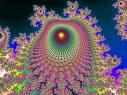
\includegraphics[width=0.60\textwidth]{images/image.jpg}
	\caption[Text im Abbildungsverzeichnis]{Text unter Abbildung}
	\label{fig:image}
\end{figure}

\section{Referenzieren}
Referenz zu einem Kapitel: \ref{sec:citation}

Referenz zu einem Bild: \ref{fig:image}

\section{Tabellen einfügen}

Schönere Tabellen als die \LaTeX-Standardtabellen lassen sich mit dem Paket {\tt booktabs} erzeugen. Dieses Paket ist in diesem Framework schon eingebunden. Ein Beispiel für eine solche schöne Tabelle zeigt Tabelle~\ref{tab:myVeryFirstTable}.

\begin{table}
	\center
	\begin{tabular}{l l l l}
		\toprule
		\bfseries{Spaltenüberschrift~1} & \bfseries{Spaltenüberschrift~2} & \bfseries{Spaltenüberschrift~3} \\
		\midrule
		Zelle~$(1,1)$                   & Zelle~$(1,2)$                   & Zelle~$(1,3)$                   \\
		Zelle~$(2,1)$                   & Zelle~$(2,2)$                   & Zelle~$(2,3)$                   \\
		Zelle~$(3,1)$                   & Zelle~$(3,2)$                   & Zelle~$(3,3)$                   \\
		\bottomrule
	\end{tabular}
	\caption
  	[Kurzer Text im Tabellenverzeichnis]
  	{Diese Tabelle kann auch etwas umfangreicher beschrieben werden. In diesem Fall bietet es sich an, für das Tabellenverzeichnis einen kürzeren Text zu definieren.}
  \label{tab:myVeryFirstTable}
\end{table}

Soll eine Zelle einer Tabelle über zwei oder mehr Zeilen laufen, bietet sich die Verwendung des Pakets {\tt multirow} an. Ein Beispiel für eine solche Tabelle zeigt Tabelle~\ref{tab:myMultiRowTable}.

\begin{table}
	\center
	\begin{tabular}{l l l l}
		\toprule
		\bfseries{Spalte~1} & \bfseries{Spalte~2} & \bfseries{Spalte~3} & \bfseries{Spalte~4} \\
		\midrule
		\multirow{2}{*}{Zelle~$\alpha$} & Zelle~$(1,2)$ & Zelle~$(1,3)$ & Zelle~$(1,4)$  \\
	                                  & Zelle~$(2,2)$ & Zelle~$(2,3)$ & Zelle~$(2,4)$  \\
		\midrule
		\multirow{2}{*}{Zelle~$\beta$}  & Zelle~$(3,2)$ & Zelle~$(3,3)$ & Zelle~$(3,4)$  \\
	                                  & Zelle~$(4,2)$ & Zelle~$(4,3)$ & Zelle~$(4,4)$  \\
		\bottomrule
	\end{tabular}
	\caption
  	{Tabelle mit {\tt multirow}s.}
  \label{tab:myMultiRowTable}
\end{table}

\section{Code einfügen}
Sourcecode lässt sich gut über die Umgebung lstlisting einfügen, man kann entweder die Sprache über lstset oder
direkt über die Umgebung setzen. Einige Optionen wie Rahmen um den Code und Zeilennummern wurden standardmäßig in der ausarbeitung.tex gesetzt. 

\lstset{language=Haskell}
\begin{lstlisting}[language=Haskell,caption=Lineare Suche]
search::Eq a => [a] -> a -> Bool
search [] _ = False
search (x:xs) a = 
	if x /= a
	then search xs a
	else True 
\end{lstlisting}

Mit lstinputlisting kann eine Sourcecode File importiert werden, über firstline und lastline kann kontrolliert werden welche Zeilen gedruckt werden.
\lstinputlisting[firstline=5,lastline=7,caption=Quicksort]{code/quicksort.hs}

\subsection{Unterabschnitt}

Lorem ipsum dolor sit amet, consetetur sadipscing elitr, sed diam nonumy eirmod tempor invidunt ut labore et dolore magna aliquyam erat, sed diam voluptua. At vero eos et accusam et justo duo dolores et ea rebum. Stet clita kasd gubergren, no sea takimata sanctus est Lorem ipsum dolor sit amet. Lorem ipsum dolor sit amet, consetetur sadipscing elitr, sed diam nonumy eirmod tempor invidunt ut labore et dolore magna aliquyam erat, sed diam voluptua. At vero eos et accusam et justo duo dolores et ea rebum. Stet clita kasd gubergren, no sea takimata sanctus est Lorem ipsum dolor sit amet.

\subsubsection{Unterunterabschnitt}

Generell sollte eine vierte Überschriftenebene wie diese hier vermieden werden.

Lorem ipsum dolor sit amet, consetetur sadipscing elitr, sed diam nonumy eirmod tempor invidunt ut labore et dolore magna aliquyam erat, sed diam voluptua. At vero eos et accusam et justo duo dolores et ea rebum. Stet clita kasd gubergren, no sea takimata sanctus est Lorem ipsum dolor sit amet. Lorem ipsum dolor sit amet, consetetur sadipscing elitr, sed diam nonumy eirmod tempor invidunt ut labore et dolore magna aliquyam erat, sed diam voluptua. At vero eos et accusam et justo duo dolores et ea rebum. Stet clita kasd gubergren, no sea takimata sanctus est Lorem ipsum dolor sit amet.

\chapter{Grundlagen}

Nach jeder Überschrift sollte ein Einleitungssatz stehen.
\section{Abschnitt}

Lorem ipsum dolor sit amet, consetetur sadipscing elitr, sed diam nonumy eirmod tempor invidunt ut labore et dolore magna aliquyam erat, sed diam voluptua. At vero eos et accusam et justo duo dolores et ea rebum. Stet clita kasd gubergren, no sea takimata sanctus est Lorem ipsum dolor sit amet. Lorem ipsum dolor sit amet, consetetur sadipscing elitr, sed diam nonumy eirmod tempor invidunt ut labore et dolore magna aliquyam erat, sed diam voluptua. At vero eos et accusam et justo duo dolores et ea rebum. Stet clita kasd gubergren, no sea takimata sanctus est Lorem ipsum dolor sit amet.

\subsection{Untersabschnitt}

Lorem ipsum dolor sit amet, consetetur sadipscing elitr, sed diam nonumy eirmod tempor invidunt ut labore et dolore magna aliquyam erat, sed diam voluptua. At vero eos et accusam et justo duo dolores et ea rebum. Stet clita kasd gubergren, no sea takimata sanctus est Lorem ipsum dolor sit amet. Lorem ipsum dolor sit amet, consetetur sadipscing elitr, sed diam nonumy eirmod tempor invidunt ut labore et dolore magna aliquyam erat, sed diam voluptua. At vero eos et accusam et justo duo dolores et ea rebum. Stet clita kasd gubergren, no sea takimata sanctus est Lorem ipsum dolor sit amet.
\chapter{Fazit}

Nach jeder Überschrift sollte ein Einleitungssatz stehen.

\section{Abschnitt}

Lorem ipsum dolor sit amet, consetetur sadipscing elitr, sed diam nonumy eirmod tempor invidunt ut labore et dolore magna aliquyam erat, sed diam voluptua. At vero eos et accusam et justo duo dolores et ea rebum. Stet clita kasd gubergren, no sea takimata sanctus est Lorem ipsum dolor sit amet. Lorem ipsum dolor sit amet, consetetur sadipscing elitr, sed diam nonumy eirmod tempor invidunt ut labore et dolore magna aliquyam erat, sed diam voluptua. At vero eos et accusam et justo duo dolores et ea rebum. Stet clita kasd gubergren, no sea takimata sanctus est Lorem ipsum dolor sit amet.

\subsection{Untersabschnitt}

Lorem ipsum dolor sit amet, consetetur sadipscing elitr, sed diam nonumy eirmod tempor invidunt ut labore et dolore magna aliquyam erat, sed diam voluptua. At vero eos et accusam et justo duo dolores et ea rebum. Stet clita kasd gubergren, no sea takimata sanctus est Lorem ipsum dolor sit amet. Lorem ipsum dolor sit amet, consetetur sadipscing elitr, sed diam nonumy eirmod tempor invidunt ut labore et dolore magna aliquyam erat, sed diam voluptua. At vero eos et accusam et justo duo dolores et ea rebum. Stet clita kasd gubergren, no sea takimata sanctus est Lorem ipsum dolor sit amet.

% Fuer einen Anhang die nachfolgenden Zeilen einkommentieren.
% \appendix
% \input{content/appendix.tex}

\cleardoublepage

%\bibliographystyle{acm}
\normalem % fix line breaks in book titles
\printbibliography

\end{document}

